\documentclass{standalone}
\usepackage{xcolor}
\usepackage{verbatim}
\usepackage[T1]{fontenc}
\usepackage{graphics}
\usepackage{hyperref}
\newcommand{\code}[1]{\texttt{#1}}
\newcommand{\R}{R}
\newcommand{\pkg}[1]{#1}
\newcommand{\CRANpkg}[1]{\pkg{#1}}%
\newcommand{\BIOpkg}[1]{\pkg{#1}}
\usepackage{amsmath,amssymb,array}
\usepackage{booktabs}
\usepackage{multicol, calc}
\usepackage{tikz}
\usetikzlibrary{patterns,positioning,babel}
\usepackage{threeparttable}
\usepackage{natbib}
\usepackage{inconsolata}
\usepackage{listings}
\usepackage{tikz-qtree}
\usepackage{subcaption} 

\begin{document}
\nopagecolor
	
        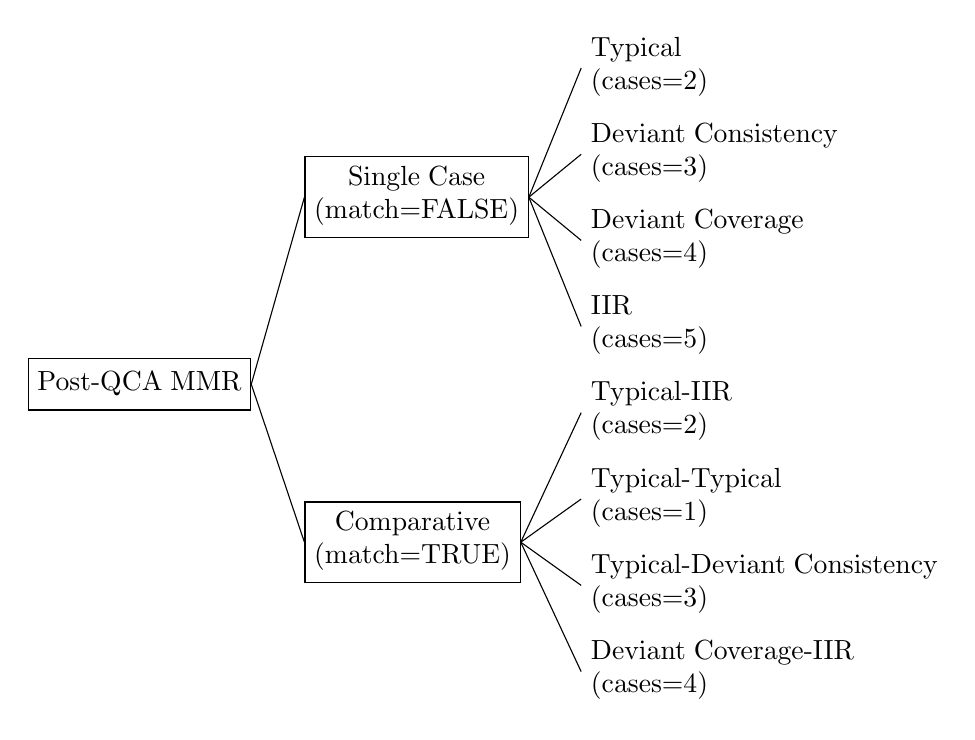
\begin{tikzpicture} [grow=right]
        \tikzset{level distance=100pt} [sibling distance=30pt]
        \tikzset{execute at begin node=\strut}
        \tikzset{every tree node/.style={anchor=base west}}
        \Tree [.\node[draw]{Post-QCA\hspace{1mm}MMR};  [.\node[draw, align=center]{Comparative\\(match=TRUE)};
                                              [.\node[align=left]{Deviant\hspace{1mm}Coverage-IIR\\(cases=4)}; ]
                                              [.\node[align=left]{Typical-Deviant\hspace{1mm}Consistency\\(cases=3)}; ]
                                              [.\node[align=left]{Typical-Typical\\(cases=1)}; ]
                                              [.\node[align=left]{Typical-IIR\\(cases=2)}; ]]
                                          [.\node[draw, align=center]{Single\hspace{1mm}Case\\(match=FALSE)};
                                              [.\node[align=left]{IIR\\(cases=5)}; ]
                                              [.\node[align=left]{Deviant\hspace{1mm}Coverage\\(cases=4)}; ]
                                              [.\node[align=left]{Deviant\hspace{1mm}Consistency\\(cases=3)}; ]
                                              [.\node[align=left]{Typical\\(cases=2)}; ]]]
        \end{tikzpicture}
\end{document}
